\chapter{Proposed solutions}\label{chap:proposed_solutions}

	Motivated by previous solutions, mentioned in Chapter \ref{chap:existing_solutions}, Sections \ref{subsec:intra_inter} and \ref{subsec:linear_geo}, we propose multiple approaches to solve the problem of tracklet building. The first one, described in Section \ref{sec:linear_regression} takes advantage of the facts mentioned in Section \ref{subsec:linear_geo}, specifically that picking sufficiently small part of the object's trajectory will make the object appear as if it moved in uniform linear motion. Section \ref{sec:IDO} describes an algorithm which filters and validates data gathered in Section \ref{sec:linear_regression}. An experimental neural network's construction and relevance is discussed in Section \ref{sec:neural} and Section \ref{sec:hough} acknowledges another possible solution which has not been implemented but has been considered nevertheless.

\section{Use of linear regression}\label{sec:linear_regression}

	Linear regression is a well-known statistical concept modelling the linear relationship between a scalar dependent variable \emph{y} and one or more independent variables, usually denoted as \emph{x}. In this thesis, we will be using a single scalar predictor variable and a single scalar response variable - simple linear regression (SLR). We chose SLR because objects in our case appear as if they followed the rules of uniform linear motion (for details on uniform linear motion, see Chapter \ref{chap:existing_solutions}, Section \ref{sec:linear_motion}). For more information about linear regression as a statistical model, see \citep{freedman2005statistical}.
	
	As discussed in Chapter \ref{chap:object_dynamics}, Section \ref{sec:ccd}, objects' position on the image reference frame in each image in the set of provided inputs (see Chapter \ref{chap:requirements}, Section \ref{sec:input_data}) are represented by the values \emph{x} and \emph{y}. The first draft of linear regression was designed and realised using these values - \emph{x} as an independent value and \emph{y} as a dependent value.
	
	To successfully create a tracklet, at least three confirmed observations out of several images are required. All objects are attempted to be classified beforehand and have several mandatory attributes assigned to them. However, some of them are unidentified or potentially misidentified (unknown) and can be the object we are looking for. 
	
	First, we pair each unknown point $p_1$ of an object $o_1$ from the first image with each unknown point $p_2$ of an object $o_2$ from the second image. Then we create a line $l$ such that $p_1,\ p_2 \in l$. The final number of existing lines after this procedure is equal to $n_1 * n_2$ where $n_1$ is the number of unknown points in the first image and $n_2$ is the number of unknown points in the second image. It is important to note that this number might be relatively high depending on the number of unknown points and therefore on the quality of the pre-processing of each image. 
	
	The point of the initial procedure described in the above paragraph is that if we removed all irrelevant points we would be left with one line placed among all the relevant points from the rest of the images (see gray and orange coloured points in Figure \ref{fig:regresia1}).
	
	However, there are several issues with this approach. First, fake objects might appear along a line in the same fashion as the real do. Second, the real points might have non-negligible distance from a line. Third, the first or second point might be deviated too - this would cause the line to have incorrect slope. Fourth, the real points might appear as if their acceleration was non-zero. 
	
	The last three problems are mainly caused by atmospheric fluctuations and errors in the CCD camera processing and the first one is the result of cosmic rays impacting the CCD arrays. We provide solutions to all of these complications in the next paragraphs.
	
	 To filter out points which have almost zero probability of being real objects we introduce a distance threshold $T_l$ which determines a maximum distance a point can have from the currently considered line. 
	
	\begin{figure}[H]
	\centering
	  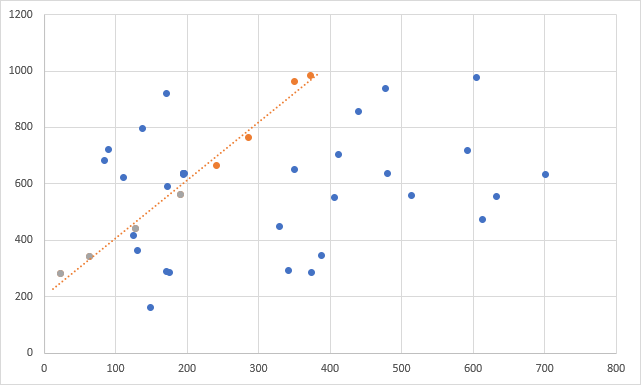
\includegraphics[width=12cm]{images/regresia1}
		  \caption{Points scattered along a trend line.}
	  \label{fig:regresia1}
	\end{figure}
	
	The distance of a point $p=(x,y)$ from the line $Am+Bn+C=0$ is calculated by using formula $$d_p=\frac{|Ax+By+C|}{\sqrt{A^2+B^2}}$$ We disregard a point if $d_p>T_l$, otherwise we process it in the next filter stage. The value of threshold $T_l$ is set manually and can be changed from one batch of images to another. The higher the value the better the chance that a possibly highly deviated point will be included for further filters at the cost of considering irrelevant points as well. To mitigate this disadvantage and improve the accuracy of the process we extend our filter by calculating angle between the currently considered point and the last probable point.
	
	Consider having two points represented by their positions $p_{i}=(x_i,y_i)$, $p_j=(x_j,y_j)$. We calculate angle $\theta$ between them as $$\theta=|\arctantwo(y_j-y_i, x_j-x_i)|$$ We then check whether the angle is within a manually set angle threshold $T_a$ which provides yet another constraint on the placement of a point in the form of a theoretical two dimensional band. Introducing this restriction is crucial for removing objects which fall within the distance threshold $T_l$ but are deviated too much. Therefore, it allows us to preserve points which conform to the line. On the other hand, setting the angle threshold $T_a$ to a redundantly high value can have negative impact on the effectiveness of the filter.
	
	\begin{figure}[H]
	\centering
	  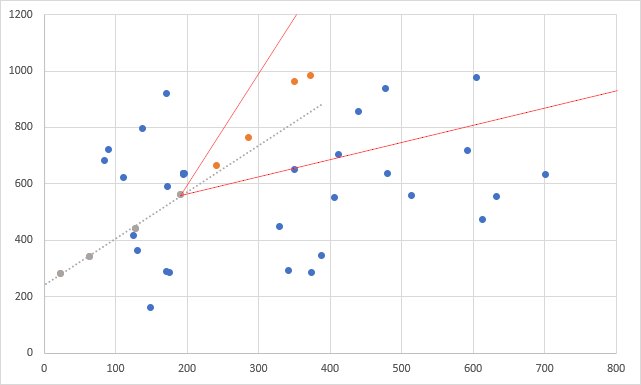
\includegraphics[width=12cm]{images/regresia2}
		  \caption{Heading of an object.}
	  \label{fig:regresia2}
	\end{figure}
		
	The last stage of the filter contains usage of speed $s$, which is calculated by using the formula $$s=\frac{d}{{\Delta}t}$$ where $d=\sqrt{(x_1-x_2)^2 + (y_1-y_2)^2}$ where $(x_1,y_1)$ and $(x_2,y_2)$ are two successive points in time and ${\Delta}t=|t_1-t_2|$. We get the time $t_{i},\ i\in\langle1,N\rangle$ where $N$ is the number of images. The purpose of the distance filter is to resolve an object's position perpendicular to its theoretical trajectory, and, to an extent, the purpose of the angle filter as well. The speed filter is mostly responsible to determine an object's position parallel to its trajectory. With regards to the previous filters we use speed threshold $T_s$ which is different for each batch of images as it describes the approximate velocity of the object.
	
	Only after each of these three filters has been satisfied by the currently chosen object $o_i$ and its point $p_i$, we add it to the list of potential candidates. 
	
	However, there is yet another metric that helps determining the most probable object for a currently constructed tracklet. Filters only select out points within user set boundaries - the candidates are then sorted by comparing the values gotten while processing filters. We treat first two objects $o_1$ and $o_2$ as a baseline - we calculate their speed and angle and then compare speed and angle of each successive object $o_i$ with the baseline. The object with the closest value is then put at the front of the list and therefore implicitly marked as the most probable real object. SLR is then calculated again, containing the last added object as well. It is important to note that we add exactly one object from every image before moving to the next image. As opposed to adding every filtered object, this has proved to be a better solution.
	
	The representation of each object $o_i$ can be specified either by the standard coordinate system in the two-dimensional Euclidean plane or by a reference system, specifically RA/Dec (see Chapter \ref{chap:object_dynamics}, Section \ref{sec:ra_dec}). The main difference and the reason why we swapped a coordinate system for a reference system is that the RA/Dec is more precise and mostly devoid of errors and deviations. The difference is best shown rather than explained - see Figure \ref{fig:regresia3}. On the left, there are shown 8 observations of the same object (an asteroid 2017\_PR25), represented in modified RA/Dec and on the right the same 8 observations, represented in the standard coordinate system. It is clearly visible that the deviation of each point in the right graph is more extreme than in the left graph. Acceleration of some of the points appears to be higher than zero - this is because the images were taken in different time intervals.
	
	\begin{figure}[H]
	\centering
	  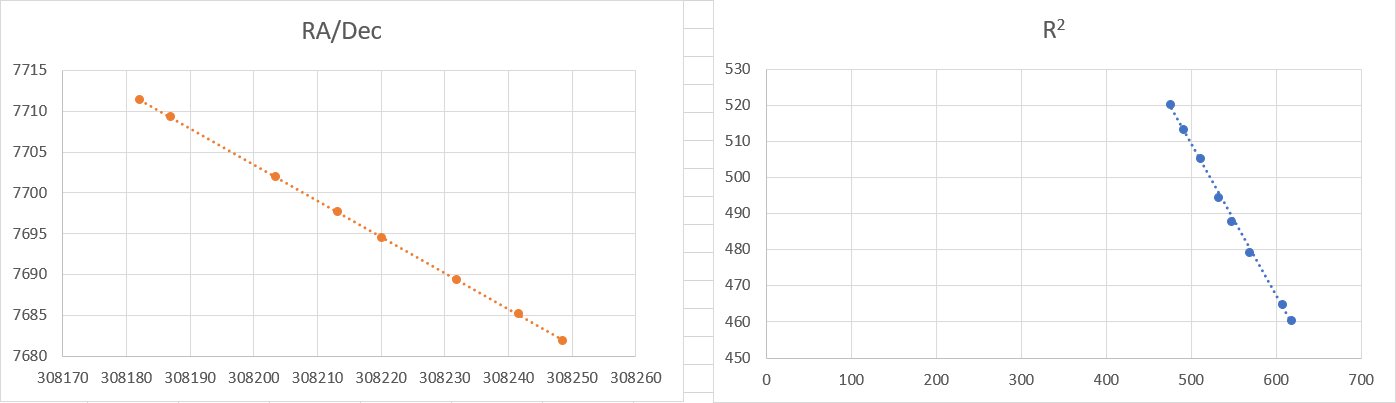
\includegraphics[width=\linewidth]{images/regresia3}
		  \caption{RA/Dec comparison.}
	  \label{fig:regresia3}
	\end{figure}
	
	We touched upon every problem mentioned before - we disregard points which are too far from the line, we correct the line by dynamically adding objects and re-calculating SLR, we filter out fake objects with nonsense speeds and angles. However, the situation when a fake object passes through all these filters and is marked as real is possible, although very improbable, and is remedied, or rather verified, by using IOD. The final result is several tracklets of unknown objects. As mentioned previously, tracklets have to contain at least three objects and thus we remove those which do not satisfy this condition.

\section{Use of the Initial Orbit Determination algorithms}\label{sec:IDO}

	The theoretical details of IOD are described in Chapter \ref{chap:object_dynamics}, Section \ref{sec:init_orbit_det}. We used a fully functional implementation of IOD from \citep{Silha2012id}.

	The provided algorithm works as a standalone program but can be wrapped in our implementation and used for verifying data we provide to it.
	
	 In order to function correctly, the algorithm requires information about the observer and three separate objects. For the observer, the information we pass is about AGO (see Chapter \ref{chap:introduction}, Section \ref{subsec:fmpi_ago}), specifically longitude and latitude in radians, and altitude. For the objects, we need to input RA in radians, Dec in radians and time of the observation in Modified Julian Date. Then the orbital elements described in Chapter \ref{chap:object_dynamics} are calculated and objects are evaluated as belonging to the same trajectory or not.
	 
	 In the vast majority of cases, we are left with more than three objects from the previous phase (Section \ref{sec:linear_regression} in this chapter). In order to check them all, we need to form all possible combinations of three out of them. 
	 	
	 To calculate all possible combinations of $r$ objects out of $n$ objects we use the provided implementation in the distribution of IOD, calculated from the formula $$C(n,r)=\frac{n!}{r!(n-r)!}$$ where $r=3$.
	 
	 As an example - 11 objects in a tracklet puts the total number of combinations and runs of IOD at $C(11,3)=165$, which is a large number in this case. 
	 
	 The results of the IOD are then output into a file and we check the presence of every observation in every combination. Observations which have the highest number of appearances have the highest probability of being a real object - on the other hand, if an observation does not appear, it is considered a not real object and does not belong into a tracklet.

\section{Use of neural network}\label{sec:neural}

	An experimental part of this thesis is the use of a neural network. We are using a popular framework \emph{tflearn}.

\section{Hough transform}\label{sec:hough}

	Hough transform is an algorithm proposed in 1962 by Paul Hough and its main purpose is to detect shapes, such as ellipses or circles. The simplest form of Hough transform is however used to detect lines.
	
	For each line defined as $r=x\cos\theta+y\sin\theta$ we associate a pair $(r,\theta)$ (also called a Hough space) where $r$ is the distance of the origin $O$ of the Euclidean space or plane to the closest point on the line and $\theta$ is the angle between the $x$ axis and the line connecting the origin with the point. See Figure \ref{fig:rtheta} for illustration of the Hough space.
	
	\begin{figure}[H]
	\centering
	  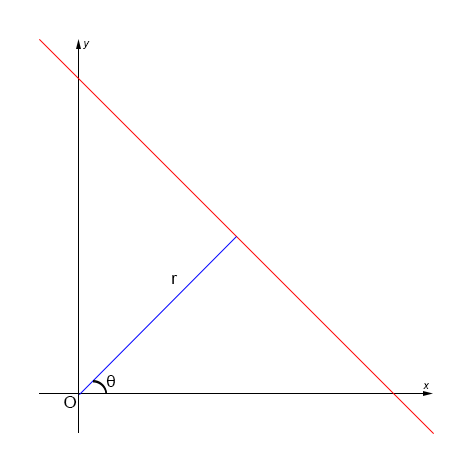
\includegraphics[width=6cm]{images/rtheta}
		  \caption{$(r,\theta)$, or Hough space visualization.}
	  \label{fig:rtheta}
	\end{figure}
	
	The principle of the transformation lies in finding unknown parameters - for a line, a two dimensional object, it's the mentioned pair $(r,\theta)$ - and plotting them from points in Cartesian space into curves in the polar Hough parameter space. Lines, which are collinear in the Cartesian space produce curves in the polar Hough parameter space and intersect at a $(r,\theta)$ point. 
	
	By forming the Hough parameter space into accumulator bins, each point in Cartesian space is transformed into a curve and bins which hold corresponding values are incremented. At the end of this procedure, bins which have the highest values represent parameters of the most likely lines.